\documentclass[10pt]{article}
\usepackage[margin=1in, paperwidth=8.5in, paperheight=11in]{geometry}
\usepackage{ifpdf,amsmath, amssymb, comment, color, graphicx, stmaryrd,setspace,enumitem,tikz, fancyhdr, wrapfig, textcomp, mathptmx, siunitx}
\usepackage{hyperref}
\hypersetup{
    colorlinks=true,
    urlcolor=blue,
}

\setlength{\headheight}{14.5pt}
\newcommand{\Q}{\mathbb{Q}}
\newcommand{\R}{\mathbb{R}}
\newcommand{\Z}{\mathbb{Z}}
\newcommand{\vu}{\mathbf{u}}
\newcommand{\vv}{\mathbf{v}}
\newcommand{\vw}{\mathbf{w}}
\newcommand{\vi}{\mathbf{i}}
\newcommand{\vj}{\mathbf{j}}
\newcommand{\vk}{\mathbf{k}}

\newcommand{\orth}{\operatorname{orth}}
\newcommand{\proj}{\operatorname{proj}}
\newcommand\dotp[1][.5]{\,\mathbin{\vcenter{\hbox{\scalebox{#1}{$\bullet$}}}}\,}

% Solution text is in red. If you want the solutions to show, remove the \iffalse from the definition of the \red command.
\newenvironment{red}{\color{red}}{\ignorespacesafterend}
\newcommand{\blue}[1]{\textcolor{blue}{#1}}
\newcommand{\green}[1]{\textcolor{green}{#1}}
\renewcommand{\section}[1]{\begin{center} \textbf{#1} \\\end{center}}
%
\hyphenpenalty=5000
\setlength{\parindent}{0in}
%\oddsidemargin=-.25in
\allowdisplaybreaks
\pagestyle{fancy}
\renewcommand{\headrulewidth}{0pt}
\lhead{MATH 203}
\rhead{Fall 2024}
%\lfoot{\copyright\ CLEAR Calculus 2010}
\cfoot{}

\begin{document}
%


%\onehalfspacing
\allowdisplaybreaks
%##################################################################
\section{PS\#2: Vectors and vector products - \red{Answer key} }

\begin{enumerate}[leftmargin=0pt]
    \item 
    \begin{minipage}[t]{0.5\linewidth}
    (ACM 9.2 Exercise 16)
    A force (like gravity) has both a magnitude and a direction. If two forces $\vu$ and $\vv$ are applied to an object at the same point, the resultant force on the object is the vector sum of the two forces. When a force is applied by a rope or a cable, we call that force \textit{tension}. Vectors can be used to determine tension.
    
    As an example, suppose a painting weighing 50 pounds is hung from a wire attached to a hook which is not perfectly centered on the picture, as illustrated in the figure. We need to know how much tension will be on the wire to know what kind of wire to use to hang the picture. Assume the hook is on the picture frame at point $O$. Let $\vu$ be the vector emanating from point $O$ to the left and $\vv$ the vector emanating from point $O$ to the right. Assume $\vu$ makes a $60^\circ$ angle with the horizontal at point $O$ and $\vv$ makes a $45^\circ$ angle with the horizontal at point $O$. Our goal is to determine the vectors $\vu$ and $\vv$.
    \end{minipage}
    \hfill
    \begin{minipage}[t]{0.4\linewidth}
    \vspace{0pt}
    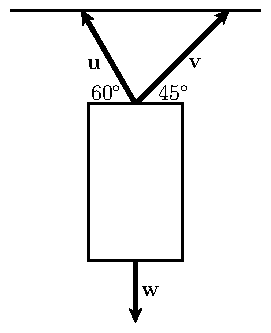
\includegraphics[width=\linewidth]{./fig_9_2_forces.pdf}
    \end{minipage}
    \begin{enumerate}
        \item Treat point $O$ as the origin. Use trigonometry to find the components $u_1$ and $u_2$ so that $\vu = u_1 \vi + u_2 \vj$. Since we don't know the magnitude of $u$, your components will be in terms of $|\vu|$ and the cosine and sine of some angle. The find the components $v_1$ and $v_2$ so that $\vv =v_1 \vi + v_2 \vj$. Again, your components will be in terms of $|\vv|$ and the cosine and sine of some angle.
        
        \begin{red}
        Note that in this situation, positive $\vi$ points to the right and positive $\vj$ points up.\\
        By trigonometry, the horizontal component of $\vu$ is $|\vu|\cos60^\circ$, and the vertical component is $|\vu|\sin60^\circ$. So, $\vu = -|\vu|\cos60^\circ \vi + |\vu|\sin60^\circ \vj$. (Note the negative sign on the first component, so that $\vu$ points left.)\\
        Similarly, $\vv = |\vv|\cos45^\circ \vi + |\vv|\sin45^\circ \vj$. (No negatives this time.)
        \end{red}
        \item The total force holding the picture up is given by $\vu + \vv$. The force acting to pull the picture down is given by the weight of the picture. Find the force vector $\vw$ acting to pull the picture down.
        
        \begin{red}
        Since the picture weighs 50 pounds, $\vw = -50\vj$. Should be negative, because the force is pointing \textbf{down}.
        \end{red}
        \item The picture will hang in equilibrium when the force acting to hold it up is equal in magnitude and opposite in direction to the force acting to pull it down. Equate these forces to find the components of the vectors $\vu$ and $\vw$.
        
        \begin{red}
        In symbols, what we want is $\vu + \vv = -\vw$, because the resultant tension force $\vu + \vv$ should act to counter the weight of the picture.
        So, we want $(-|\vu|\cos60^\circ \vi + |\vu|\sin60^\circ \vj) + (|\vv|\cos45^\circ \vi + |\vv|\sin45^\circ \vj) = 0 \vi + 50 \vj$. Equating the $\vi$ and $\vj$ components:
        \begin{align*}
            -|\vu|\cos60^\circ + |\vv|\cos45^\circ &= 0 \\
             |\vu|\sin60^\circ + |\vv|\sin45^\circ &= 50
        \end{align*}
        Now we have a system of two equations in two unknowns, $|\vu|$ and $|\vv|$. The solution of this system will require some tedious algebra, which I'm happy to feed to Wolfram$|$Alpha (using $u$ to mean $|\vu|$ and similar for $v$):
        \\
        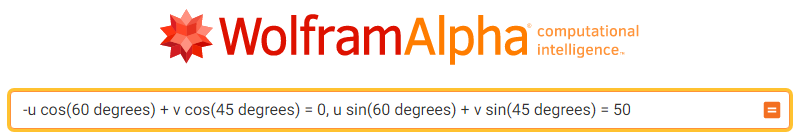
\includegraphics[width=\linewidth]{wa-3-1.png} \\
        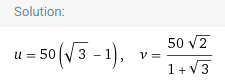
\includegraphics[width=0.4\linewidth]{wa-3-2.png}
        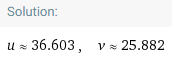
\includegraphics[width=0.4\linewidth]{wa-3-3.png}\\
        Thanks, Wolfram$|$Alpha! Therefore:
        \begin{align*}
            \vu &= - 50(\sqrt{3} - 1) \cos60^\circ \vi + 50(\sqrt{3} - 1) \sin60^\circ \vj\\
            &\approx -18.301 \vi + 31.699 \vj \\
            \vv &= \frac{50\sqrt{2}}{1+\sqrt{3}}\cos45^\circ\vi + \frac{50\sqrt{2}}{1+\sqrt{3}}\sin45^\circ\vj\\
            &\approx 18.301 \vi + 18.301 \vj.
        \end{align*}
        You can check that $\vu$ and $\vv$ do in fact add up to $50\vj$.
        \end{red}
    \end{enumerate}
    
    \item In one of the WeBWorK problems, it talks about the orthogonal component of $\vu$ onto $\vv$:
		$\orth_\vv \vu = \vu - \proj_\vv \vu$.
		The idea is that the vector projection of $\vu$ onto $\vv$ is certainly parallel to $\vv$, so if we subtract that from $\vu$, we'll end up with exactly the part of $\vu$ that's orthogonal to $\vv$. Your job in this problem is to prove to me that this actually works: show, for some generic vectors $\vu$ and $\vv$ that $\orth_\vv \vu$ is indeed orthogonal to $\vv$.
		
		\begin{red}
			We can tell two vectors are orthogonal if their dot product is zero. So, let's compute $(\orth_\vv \vu) \dotp \vv$ and see if we get $0$ like we want:
			\begin{align*}
				(\orth_\vv \vu) \dotp \vv &= (\vu - \proj_\vv \vu) \dotp \vv 
				= \left(\vu - \frac{\vu\dotp\vv}{|\vv|^2}\vv \right) \dotp \vv \\
				&= \vu \dotp \vv - \left(\frac{\vu\dotp\vv}{|\vv|^2}\right)\vv\dotp\vv \\
				\intertext{Now, note that the dot product of a vector with itself is the magnitude of that vector, squared:}
				&= \vu \dotp \vv - \left(\frac{\vu\dotp\vv}{|\vv|^2}\right)|\vv|^2\\
				&= \vu \dotp \vv - \vu \dotp \vv = 0
			\end{align*}
			Hooray, we're orthogonal.
		\end{red}
	\item 
    \begin{minipage}[t]{0.5\linewidth}
    Molecular geometry is the geometry determined by arrangements of atoms in molecules. Molecular geometry includes measurements like bond angle, bond length, and torsional angles. These attributes influence several properties of molecules, such as reactivity, color, and polarity.
    
    As an example of the molecular geometry of a molecule, consider the methane CH$_4$ molecule, as illustrated in the figure to the right . According to the Valence Shell Electron Repulsion (VSEPR) model, atoms that surround single different atoms do so in a way that positions them as far apart as possible. This means that the hydrogen atoms in the methane molecule arrange themselves at the vertices of a regular tetrahedron. The bond angle for methane is the angle determined by two consecutive hydrogen atoms and the central carbon atom. 
    \end{minipage} 
    \hfill
    \begin{minipage}[t]{0.49\linewidth}
    \vspace{0pt}
    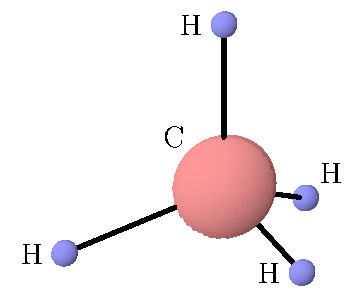
\includegraphics[width=\textwidth]{./fig_9_3_methane.pdf}
    \end{minipage}
    
    To determine the bond angle for methane, we can place the center carbon atom at the point $\left(\frac{1}{2},\frac{1}{2},\frac{1}{2}\right)$ and the hydrogen atoms at the points $(0,0,0)$, $(1,1,0)$, $(1,0,1)$, and $(0,1,1)$. Find the bond angle for methane to the nearest tenth of a degree.
    
    \begin{red}
    (Seeing why these are reasonable coordinates for the hydrogen atoms is a little tricky, precisely because visualizing things in 3D space is hard. I thus turned to my favorite tool, \end{red} \href{https://www.monroecc.edu/faculty/paulseeburger/calcnsf/CalcPlot3D/?type=point;point=(1/2,1/2,1/2);visible=true;color=rgb(255,0,0);size=4&type=point;point=(0,0,0);visible=true;color=rgb(17,109,192);size=6&type=point;point=(1,1,0);visible=true;color=rgb(17,109,192);size=6&type=point;point=(1,0,1);visible=true;color=rgb(17,109,192);size=6&type=point;point=(0,1,1);visible=true;color=rgb(17,109,192);size=6&type=window;hsrmode=3;nomidpts=false;anaglyph=-1;center=3.0188813072265694,9.378882675117357,5.056037826737073,1;focus=1,1,1,1;up=0.17012619465221945,-0.4273100550319643,0.8879545003893696,1;transparent=false;alpha=140;twoviews=false;unlinkviews=false;axisextension=0.7;xaxislabel=x;yaxislabel=y;zaxislabel=z;edgeson=true;faceson=true;showbox=true;showaxes=true;showticks=true;perspective=true;centerxpercent=0.5;centerypercent=0.5;rotationsteps=30;autospin=true;xygrid=false;yzgrid=false;xzgrid=false;gridsonbox=true;gridplanes=false;gridcolor=rgb(128,128,128);xmin=0;xmax=2;ymin=0;ymax=2;zmin=0;zmax=2;xscale=1;yscale=1;zscale=1;zcmin=-2;zcmax=4;zoom=1.773333;xscalefactor=1;yscalefactor=1;zscalefactor=1}{CalcPlot3D}.
    \begin{red} Click on that link and it'll take you to a pre-set graph with the points all typed in and everything.)
    
    So here's what we need to do: we need to find vectors from the central carbon atom out to two of the hydrogen atoms, and call the vectors $\vu$ and $\vv$. Then the dot product of those vectors will be $|\vu|\cdot|\vv|\cdot\cos\theta$, where $\theta$ is the angle we're interested in. Then some inverse trig will get us the angle we want.
    
    It doesn't really matter which two hydrogen atoms you pick to be your vector ends. I'll just pick $(0,0,0)$ and $(1, 1, 0)$. 
    
    The first vector $\vu$ should go \textbf{from} $\left(\frac{1}{2},\frac{1}{2},\frac{1}{2}\right)$  \textbf{to} $(0,0,0)$, so:
    \[\vu = \left\langle 0 - \frac{1}{2}, 0 - \frac{1}{2}, 0 - \frac{1}{2} \right\rangle = \left\langle -\frac{1}{2},-\frac{1}{2},-\frac{1}{2}\right\rangle.\]
    Similarly, 
    \[\vv = \left\langle 1-\frac{1}{2}, 1-\frac{1}{2}, 0-\frac{1}{2}\right\rangle = \left\langle \frac{1}{2},\frac{1}{2},-\frac{1}{2}\right\rangle.\]
    The magnitudes $|\vu|$ and $|\vv|$ are the same: 
    \[\vu = \vv = \sqrt{\left(\frac{1}{2}\right)^2 + 
    \left(\frac{1}{2}\right)^2 + 
    \left(\frac{1}{2}\right)^2} = \sqrt{\frac{3}{4}} = \frac{\sqrt{3}}{2}.\]
    Computing the dot product:
    \[\vu \dotp \vv = -\frac{1}{4} - \frac{1}{4} + \frac{1}{4} = -\frac{1}{4}.\]
    Now we have all the pieces we need:
    \begin{align*}
        \vu\dotp\vv &= |\vu| \cdot |\vv| \cdot \cos\theta \\
        -\frac{1}{4} &= \frac{\sqrt{3}}{2} \cdot \frac{\sqrt{3}}{2} \cdot \cos\theta \\
        -\frac{1}{4} &= \frac{3}{4} \cos\theta \\
        -\frac{1}{4}\cdot\frac{4}{3} &= \cos\theta \\
        \arccos \left(-\frac{1}{3}\right) &= \theta \\
        \theta &\approx 109.5^\circ
    \end{align*}
    A quick google confirms that we've landed on the right answer according to like Wikipedia or whatever. Yay!
    \end{red}
\end{enumerate}

\end{document}